\chapter{Információs technológiai infrastruktúrák}

Ebben a részben néhány skálázási és nagy rendelkezésre állást biztosító technikát mutatok be, majd néhány szóban a virtualizációt jellemzem, végül a felhőalapú infrastruktúrát, annak tulajdonságait, szolgáltatásait részletezem.

\section{A klasszikus IT infrastruktúra}
A klasszikusnak mondott háromrétegű IT infrastruktúrát az írás korábbi részében már bemutattam. Itt most az architektúra egyes rétegeinek skálázását, megbízhatósági szintjének növelésére adott lehetőségeket szeretném bemutatni.
\subsection{Adatbázis réteg}
Az adatbázis réteg skálázása és megbízhatósági szintjének, rendelkezésre állásának növelése megoldott probléma, hiszen az iparban az egyik legrégebben és leggyakrabban alkalmazott szolgáltatások közé tartoznak az adatbázis szerverek. A piacon található adatbáziskezelő-rendszerek nagy része rendelkezik beépített vagy külső technológiákkal.
Az adatbázisok esetében három eltérő megvalósítást szoktak alkalmazni, amelyek\cite{mizofr}:
\begin{sajat_itemize}
\item terheléselosztás (\angolul{load balancing}),
\item replikálás,
\item feladatátadás hiba esetén (\angolul{failover}).
\end{sajat_itemize}

\subsubsection{Terheléselosztás (\angolul{load balancing})}

Az adatbázisszerverek képesek együttműködni abból a célból, hogy csökkentség az egy példányra jutó kérések számát. Az úgynevezett terheléselosztás azt jelenti, hogy egy hardver vagy szoftver elem az adatbázisréteghez beérkező tranzakciókat valamilyen algoritmus (pl. \angolul{round-robin} vagy bonyolultabb megoldások) szerint szétosztja a szerver példányok között. Ennél a technikánál a rétegen kívüli részvevőknek úgy tűnik, mintha az egyetlen adatbázisszerver a terheléselosztó lenne.

A terheléselosztás megvalósítása nem egyszerű adatbázisok esetén, hiszen a szerver példányoknak ugyanazt az adathalmazt kell kezelniük. Csak olvasás esetén ez nem jelent problémát, mivel minden szerver példány ugyanazzal az adattal rendelkezik, ebből kifolyólag a terheléselosztó bármelyiknek is küldi tovább a kérést, ugyanazt az adatot fogja visszaadni.
Írási műveletek esetén már bonyolultabb a megvalósítás, hiszen a kérés eredményének valamilyen megoldással minden egyes szerver példányhoz el kell jutnia. Erre különböző szinkronizálási technikák alkalmazhatók, amelyeket most itt nem áll szándékomban részletezni.

\subsubsection{Replikálás}

A replikálás alapvetően abban különbözik az előbb említett terheléselosztásos technikától, hogy a rétegen kívüli szereplők minden egyes szerverpéldányról tudnak. Itt is lényeges a szinkronizáció megvalósítása.

Léteznek olyan megoldások, amelyeknél csak az egyik szerverpéldány (\angolul{master}) fogadja az írási műveleteket, amelyeket \angolul{push} vagy \angolul{pull} szinkronizációval kap meg a többi szerver (\angolul{slave}), míg az olvasási műveletekre nincs ilyen megkötés.

Az ún. \angolul{multimaster} megoldás esetén minden példány írható és olvasható is, ám ekkor sokkal bonyolultabb a szinkronizáció megvalósítása.

\subsubsection{Feladatátadás hiba esetén (\angolul{failover})}

A feladatátadás egy olyan technika, amelynek során bármilyen szoftveres/hardveres hiba vagy rendellenes működés esetén az egyik erőforrástól egy redundáns vagy készenléti erőforrás automatikusan, esetleg manuálisan átveszi az adott feladat végrehajtását.

Az egyes szerverek között egy állandó kapcsolat (,,\angolul{heartbeat}'') található. Amennyiben az egyik szerver oldaláról megszűnne a ,,\angolul{heartbeat}'', úgy a másik amilyen hamar csak lehetséges, átveszi a meghibásodott kiszolgáló feladatát. Mihelyt a kiesett szerver újra működőképes, a másodlagos szerver visszaadhatja neki a feladat végrehajtásának jogát.

\subsection{Alkalmazás réteg}

Mivel az alkalmazás réteg sokszor hardver szinten nem válik szét a webkiszolgáló rétegtől, azért a következőekben ott bemutatott technikákat lehet használni ennek a rétegnek az esetében is.
Viszont ennek a rétegnek van egy olyan tulajdonsága skálázási szempontból, amely nem kezelhető az üzemeltetési oldalról, ez pedig magának az alkalmazásnak a skálázhatósága, vagyis hogy a fejlesztett program mennyire ad lehetőséget arra, hogy skálázható legyen.

\subsection{Webkiszolgáló réteg}

A webkiszolgáló réteg rendelkezésre állásának növelésére az egyik leggyakoribb megoldás a terheléselosztás. Erre az egyik technika az ún. RRDNS, vagy Round-robin Domain Name Service. Lényege, hogy az oldalunkhoz kapcsolódó DNS bejegyzéshez több IP tartozik, mégpedig a webkiszolgáló példányaink számával megegyező. Így minden egyes DNS feloldás eredménye eltérő IP-cím lesz a round-robin működésnek megfelelően, ezért a webszerverek közel egyenlő módon lesznek terhelve.

A megoldás előnye, hogy rugalmasan skálázható, hiszen webkiszolgálókat elvehetünk és hozzáadhatunk a rendszerhez anélkül, hogy ebből a külvilág bármit is észrevenne. Hátránya, hogy a DNS szerver esetlegesen SPOF-ként (\angolul{Single Point of Failure}) viselkedhet, hiszen kiesése esetén a kérések nem jutnak el a webszervereinkhez. Természetesen a DNS szerverek példányszámának növelésével ez a probléma megoldható.

Az előző megoldásnál fontos, hogy ugyanaz a kliens ugyanahhoz a szerverhez kapcsolódjon egy \angolul{session} ideje alatt, kivéve ha a \angolul{session} kezelés az adatbázisrétegben kerül megvalósításra.
Erre a problémára nyújthat megoldást például az Apache (\href{https://httpd.apache.org/}{https://httpd.apache.org/}) webszerver beépített \textit{mod\_proxy\_balancer} modulja, amely kezeli ezeket a sessionöket, és terheléselosztást is megvalósít. Természetesen nem csak az Apache, de például a lighttpd (\href{http://www.lighttpd.net}{http://www.lighttpd.net}) és a nginx (\href{http://www.nginx.org/}{http://www.nginx.org/}) is rendelkezik beépített load balancing funkciókkal.

Természetesen az itt felsorolt különböző technikai megvalósítások koránt sem jelentik a teljes listát, nem is részleteztem teljes mélységükben őket, csak a három alapvető koncepciót mutattam be.

\section{Virtualizáció}

\todo{Megírni}

\section{Felhőalapú infrastruktúrák}

A ,,számítási felhő'' (angolul \angolul{cloud computing}) egy modell kényelmes, hálózaton keresztül hozzáférhető, konfigurálható számítási erőforrások (pl. hálózat, szerverek, tárhelyek, alkalmazások és szolgáltatások) egy megosztott készletének elérhetőségére, mely erőforrásokat minimális intézkedési erőfeszítéssel vagy szolgáltatói közbenjárással gyorsan rendelkezésre lehet bocsátani \cite{nistsp800-145}.

\begin{comment}
Cloud computing is a model for enabling ubiquitous, convenient, on-demand network access to a shared pool of configurable computing resources (e.g., networks, servers, storage, applications, and services) that can be rapidly provisioned and released with minimal management effort or service provider interaction. 
\end{comment}

Általában hivatkozás szintjén nincsenek elkülönítve az Interneten keresztül szolgáltatott alkalmazások és a felhő infrastrukturális részét képező hardverek, szoftverek, amelyek ezeket az alkalmazásokat elérhetővé teszik. Ahogy azt \aref{fig:cloud_computing_hu}.~ábrán is szemléltetni próbálom, a felhő részét képezi az alkalmazás, szolgáltatás és a hardver is.

\begin{figure}[h!]
\centering
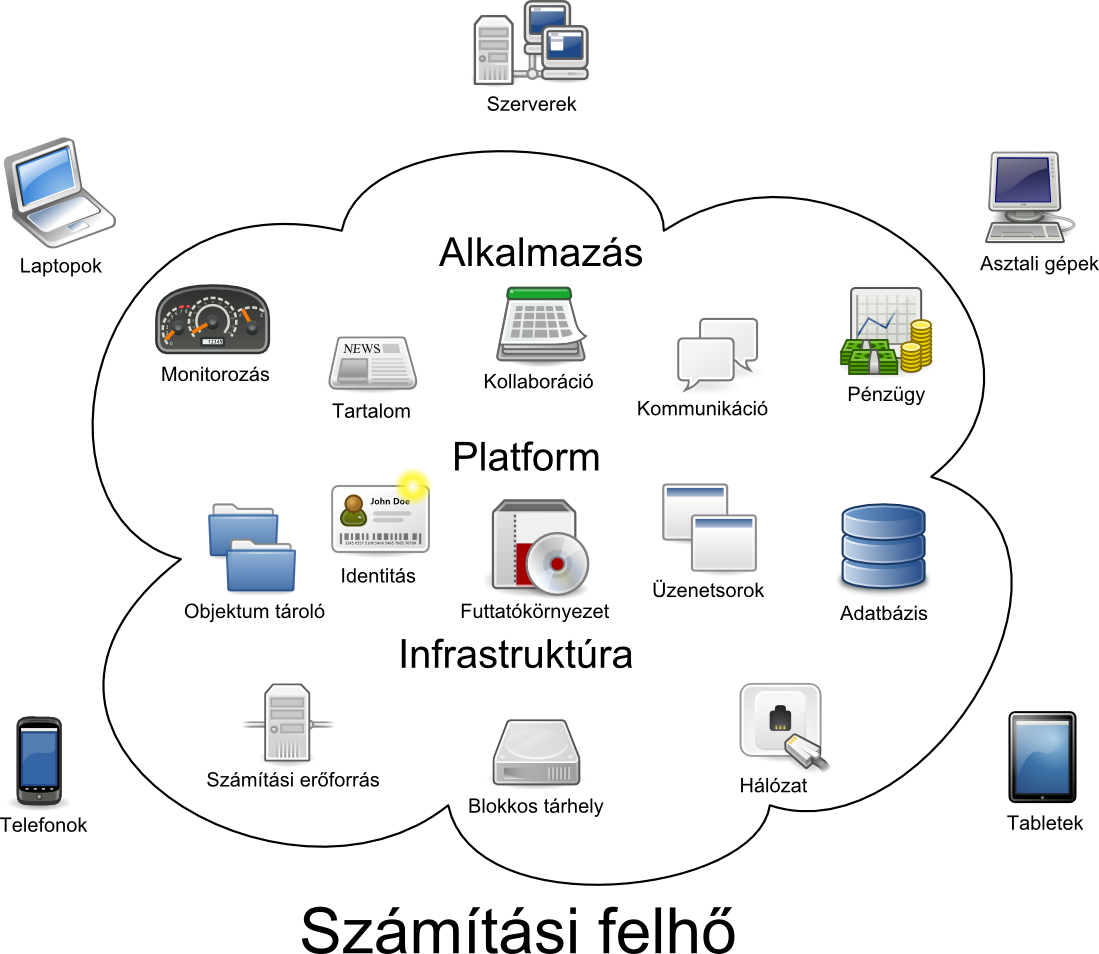
\includegraphics[width=0.80\textwidth]{figures/Cloud_computing_hu.png}
\caption{A számítási felhő (\angolul{cloud computing}) (Forrás: \href{https://en.wikipedia.org/wiki/File:Cloud\_computing.svg}{Wikipedia})} \label{fig:cloud_computing_hu}
\end{figure}

\subsection{A felhők alapvető jellemzői}
A felhőkkel kapcsolatban az irodalom\cite{nistsp800-145} öt alapvető tulajdonságot, jellemzőt szokott felhozni. Ezeket szeretném most összegyűjteni, és néhány szóban leírni.
 
\subsubsection{Igény szerinti önkiszolgálás (\angolul{On-demand self-service})}

\begin{comment}
\angolul{''A consumer can unilaterally provision computing capabilities, such as server time and network storage, as needed automatically without requiring human interaction with each service provider.''}\cite{nistsp800-145}
\end{comment}

Az előfizető vagy felhasználó egyoldalúan tudja akár automatikusan módosítani a számítási kapacitást, pl. a processzoridőt és hálózati tárhelyet, amint arra szükség van, emberi interakció nélkül.

\subsubsection{Széleskörű hálózati elérés (\angolul{Broad network access})}

\begin{comment}
\angolul{''Capabilities are available over the network and accessed through standard mechanisms that promote use by heterogeneous thin or thick client platforms (e.g., mobile phones, tablets, laptops, and workstations).''}\cite{nistsp800-145}
\end{comment}

Az erőforrások elérhetőek a hálózaton, és hozzáférhetőek olyan szabványos mechanizmusokon keresztül, amelyek támogatják heterogén vékony- vagy vastagkliens platformok (pl. mobiltelefonok, tabletek, laptopok és munkaállomások) használatát.

\subsubsection{Erőforrás készletezés (\angolul{Resource pooling})}

\begin{comment}
\angolul{''The provider’s computing resources are pooled to serve multiple consumers using a multi-tenant model, with different physical and virtual resources dynamically assigned and reassigned according to consumer demand. There is a sense of location independence in that the customer generally has no control or knowledge over the exact location of the provided resources but may be able to specify location at a higher level of abstraction (e.g., country, state, or datacenter). Examples of resources include storage, processing, memory, and network bandwidth.''}\cite{nistsp800-145}
\end{comment}

A szolgáltató számítási erőforrásai egy készletben találhatók, több előfizető egyszerre történő kiszolgálására egy többszörös-bérlő (multi-tenant) modellt használnak, amely modellel különböző fizikai és virtuális erőforrásokat dinamikusan kioszthatnak vagy újraoszthatnak az előfizető igényeinek megfelelően. Megjelenik a helyfüggetlenség fogalma, vagyis hogy a felhasználó általánosan nem rendelkezik tudással vagy befolyásolási lehetőséggel a biztosított erőforrás helyét illetően, de lehetséges a hely meghatározása egy magasabb absztrakcióban (pl. megye, állam vagy adatközpont). Az erőforrások magukba foglalják a tárhelyet, processzoridőt, memóriát és hálózati sávszélességet.

\subsubsection{Gyors le- és felskálázódás (\angolul{Rapid elasticity})}

\begin{comment}
\angolul{''Capabilities can be elastically provisioned and released, in some cases automatically, to scale rapidly outward and inward commensurate with demand. To the consumer, the capabilities available for provisioning often appear to be unlimited and can be appropriated in any quantity at any time.''}\cite{nistsp800-145}
\end{comment}

Az erőforrások rugalmasan elérhetők és visszaadhatók, néhány esetben automatikusan, gyorsan skálázódva a külső és belső igénnyel összemérhetően. A felhasználónak a tartalékként elérhető erőforrások gyakran végtelennek tűnnek, és kisajátíthatóak bármilyen mennyiségben, bármelyik időpillanatban.

\subsubsection{Mért szolgáltatások (\angolul{Measured service})}

\begin{comment}
\angolul{''Cloud systems automatically control and optimize resource use by leveraging a metering capability at some level of abstraction appropriate to the type of service (e.g., storage, processing, bandwidth, and active user accounts). Resource usage can be monitored, controlled, and reported, providing transparency for both the provider and consumer of the utilized service.''}\cite{nistsp800-145} 
\end{comment}

A felhőalapú rendszerek mérések által befolyásolva automatikusan szabályozzák és optimalizálják az erőforrás használatot az absztrakció valamely a szolgáltatás típusának (pl. tárhely, processzoridő, sávszélesség és aktív felhasználói fiókok) megfelelő szintjén. Az erőforrás felhasználások monitorozhatóak, kontrollálhatóak és jelenthetőek, átláthatóságot nyújtva a használt szolgáltatásról mind a szolgáltatónak, mind az előfizetőnek.

Mélyebb elemzés során azonban a felhőt szolgáltatási modellekre lehet bontani, amely modelleket a következő alfejezetben részletezem.

\subsection{A felhő szolgáltatási modelljei}

A felhő napjainkban négy szolgáltatási modellt tartalmaz, amelyek valamilyen szinten egymásra épülnek, ám nem feltétlenül határolhatóak el egzaktul egymástól. \Aref{fig:cloud_retegek}.~ábrán a felhő megoldások egy réteges felosztása látható, amely körülbelül azt hivatott kifejezni, hogy alulról fölfelé hogyan csökken a szolgáltatások felhasználó által felügyelendő része.

\todo{Ábrákat megigazítani}

\begin{figure}[h!]
\centering
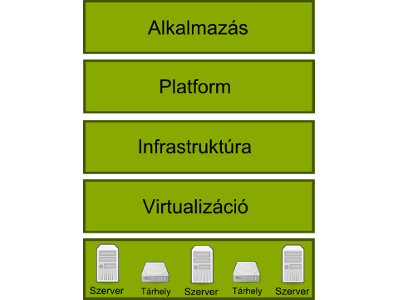
\includegraphics[width=0.25\textwidth]{figures/cloud_retegek.png}
\caption{A számítási felhő rétegei \label{fig:cloud_retegek}}
\end{figure}

A négy szolgáltatási modell és néhány hozzájuk kapcsolódó szolgáltató cég logója látható \aref{fig:cloud_service_models}.~ábrán.

\begin{figure}[h!]
\centering
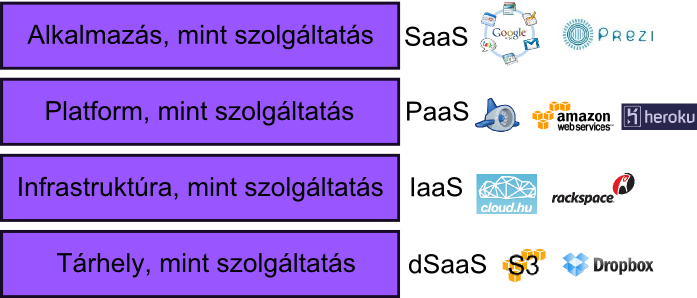
\includegraphics[width=0.5\textwidth]{figures/cloud_service_models.png}
\caption{A számítási felhő szolgáltatási modelljei \label{fig:cloud_service_models}}
\end{figure}
 
\subsubsection{Tárhely mint szolgáltatás (\angolul{data-Storage-as-a-Service, dSaaS})}
Ezt a szolgáltatást nem minden irodalom szokta említeni, ám én itt mégis külön kezelném, hiszen ez a felhő legalapvetőbb szolgáltatása. Lényege, hogy online tárhelyet biztosít a felhasználóknak. Ilyen szolgáltatást nyújt pl. a \href{http://www.dropbox.com}{Dropbox.com} (főleg személyes felhasználásra, biztonsági mentés, megosztás céljából) vagy az \href{https://aws.amazon.com/s3/}{Amazon S3} (inkább nagy szolgáltatók használják).

A dSaaS oktatási rendszerek esetében sok nagyméretű adat esetén lehet előnyös, hiszen nem kell a saját szerverünkön tárolni ezeket, megspórolva ezzel saját adattároló rendszer kialakítását, üzemeltetését. Érdemes megjegyezni, hogy sok adatpéldány esetén is érdemes lehet hasonló szolgáltatás használata, hiszen ebben az esetben az autentikációhoz kötött adatoknál már nem kell a session-öket kezelni, az adatok elérhetőségét megadó URL már tartalmaz egy kódot, csökkentve ezzel a web- és alkalmazásszerver terhelését. 

A dSaaS segítségével a rendszerünk tárhelye jól skálázható, hiszen igény esetén transzparens módon tudjuk növelni, vagy költségcsökkentés céljából visszaadni az erőforrásokat. 

\subsubsection{Infrastuktúra mint szolgálatás (\angolul{Infrastructure-as-a-Service, IaaS})}

\begin{comment}
\angolul{''The capability provided to the consumer is to provision processing, storage, networks, and other fundamental computing resources where the consumer is able to deploy and run arbitrary software, which can include operating systems and applications. The consumer does not manage or control the underlying cloud infrastructure but has control over operating systems, storage, and deployed applications; and possibly limited control of select networking components (e.g., host firewalls).''}\cite{nistsp800-145}
\end{comment}

Az infrastruktúra mint szolgáltatás az előfizető számára rendelkezésre bocsájt olyan feldolgozási, tárhely, hálózati és egyéb alapvető számítási erőforrásokat, ahol az előfizető képes telepíteni és futtatni tetszőleges szoftvert, amely szoftver magába foglalhatja magát az operációs rendszert és egyéb alkalmazásokat is. Az előfizető nem kezeli a szolgáltatás alapjául szolgáló infrastruktúrát, de irányítása alá tartozik az operációs rendszer, a tárhely és a telepített alkalmazások; esetleg korlátozottan hálózati komponensek (pl. tűzfalak)\cite{nistsp800-145}.

Az IaaS az infrastruktúra (számítási erőforrások és tárhely) bérbeadása. Ez nem csak virtualizált számítógépeket jelent garantált számítási teljesítménnyel, de fenntartott sávszélességet a tárhely és az internetelérésnek is. Ez lényegében egy számítógép vagy adatközpont bérbevételének lehetőségét jelenti, specifikált szolgáltatásminőség (QoS) megkötésekkel, amelyekkel képesek vagyunk egy tetszőleges operációs rendszer és szoftver futtatására\cite{ccwlinux}.

A legismertebb IaaS szolgáltatók az Amazon (Amazon EC2: \href{https://aws.amazon.com/ec2/}{https://aws.amazon.com/ec2/}) és a Rackspace (\href{http://www.rackspace.com/}{http://www.rackspace.com/}). A különböző IaaS-t nyújtó cégek szolgáltatásai nagyjából hasonlóak. A felhasználók előre beállított konfigurációk közül választhatják ki a nekik megfelelőt. Ezek a konfigurációk erőforrásokban, előre telepített operációs rendszerekben\footnote{Nem csak ingyenes OS-eket, de fizetős (pl. Microsoft) termékeket is igénybe vehetünk, ahol a licenc ára a felhasználás idejének arányában oszlik el, így nekünk nem kell foglalkoznunk a szoftver beszerzésével.} és árban különbözhetnek.

Egy LMS üzemeltetésével foglalkozó szervezet esetén rengeteg előnyt jelenthet a rendszer felhőben való üzemeltetése. Az IaaS elasztikus tulajdonságának köszönhetően gyorsan tudjuk a változó erőforrásigényeket kielégíteni. Ezek a szolgáltatások idő- és teljesítményalapú számlázást használnak, így jó közelítéssel előre meghatározhatóak a költségek. A szolgáltatók nagy rendelkezésre állást biztosítanak, így nem fordulhat elő, hogy a rendszerünk nem érhető el. Természetesen ezen a szinten még szükségünk van IT munkatársakra, hiszen a rendszert fel kell építeni, és szoftveres szinten karban kell tartani, de már a hardveres szint hiánya is egyszerűsítheti a munkát.

Mivel általában a szolgáltatók nem adnak lehetőséget az egyes erőforrások változtatására (pl. csak CPU vagy memória növelése, csökkentése), ezért 
az IaaS skálázási lehetősége szerver példányok hozzáadásával vagy elvételével valósítható meg.
\subsubsection{Platform mint szolgáltatás (\angolul{Platform-as-a-Service, PaaS})}

\begin{comment}
\angolul{''The capability provided to the consumer is to deploy onto the cloud infrastructure consumer-created or acquired applications created using programming languages, libraries, services, and tools supported by the provider. This capability does not necessarily preclude the use of compatible programming languages, libraries, services, and tools from other sources. The consumer does not manage or control the underlying cloud infrastructure including network, servers, operating systems, or storage, but has control over the deployed applications and possibly configuration settings for the application-hosting environment.''}\cite{nistsp800-145}
\end{comment}

A platform, mint szolgáltatás az előfizető számára rendelkezésre bocsájtja annak a lehetőségét, hogy olyan a felhasználó által létrehozott vagy beszerzett alkalmazásokat telepítsen a felhő infrastruktúrára, amelyek a szolgáltató által támogatott programozási nyelvet, könyvtárakat, szolgáltatásokat és eszközöket használnak. Ezen felül nincs kizárva  annak a lehetősége, hogy az előfizető más forrásból származó kompatibilis programozási nyelveket, könyvtárakat, szolgáltatásokat és eszközöket használjon. A felhasználó nem kezeli vagy vezérli a szolgáltatás alapjául szolgáló infrastruktúrát, beleértve a hálózatot, szervereket, operációs rendszereket vagy a tárhelyet, de irányítással rendelkezik a telepített alkalmazások és esetleg a konfigurációs beállítások felett\cite{nistsp800-145}.

A PaaS hasonló az IaaS-hoz, de olyan operációs rendszereket és kötelező szolgáltatásokat foglal magába, amelyek egy sajátos alkalmazásra fókuszálnak. Például PaaS-ként tekinthetünk egy virtualizált szerver, tárhelyszolgáltatás, operációs rendszer és alkalmazás halmazt (ami tipikusan egy virtuális gép fájl formátumban, pl. a VMware .vmdk állománya), hozzáféréssel a szükséges szolgáltatásokhoz, mint amilyen például egy MySQL adatbázis vagy egyéb, specializált helyi erőforrás. Más szavakkal a PaaS egy IaaS, testre szabott szoftver stackkel egy adott alkalmazáshoz\cite{ccwlinux}.

A piacon több PaaS szolgáltató találunk, ezek közül szedtem össze néhányat \aref{tab:paas_providers}.~táblázatba.

\begin{table}[h]
	\caption{Néhány ismertebb PaaS szolgáltató}
	\centering
	\small
	\begin{tabular}{| p{4cm} | p{5.5cm} | p{4cm} |}
		\hline
		\rowcolor{MyTableColor} \textbf{Szolgáltató} & \textbf{URL} & \textbf{Platform} \\
		\hline
		Google AppEngine & \href{https://appengine.google.com}{https://appengine.google.com} & Python, Java, Go \\ 
		\hline
		Heroku & \href{http://www.heroku.com/}{http://www.heroku.com/} & Ruby, Node.js, Clojure, Java, Python, Scala \\
		\hline
		Epio & \href{https://www.ep.io/}{https://www.ep.io/} & Python (Django, Pylons, Pyramid, Flask, Trac) \\
		\hline
		Zend PHP Cloud Application Platform & \href{http://www.zend.com/en/products/php-cloud/}{http://www.zend.com/en/products/php-cloud/} & PHP\\
		\hline
		SpringSource & \href{http://www.springsource.com/}{http://www.springsource.com/} & Java (Groovy, Grails)\\
		\hline
	\end{tabular}
	\normalsize
	\label{tab:paas_providers}
\end{table}
 

\todo{A többiről is írni pár szót!}

A Zend PHP Cloud Application Platform nem igazi szolgáltatás, csak egy platform, amelyet pl. Amazon EC2-re lehet telepíteni, mint ahogy a SpringSource is szintén egy telepíthető platform VMware vFabric Cloud Application Platform alapokon.

A PaaS egy környezetet biztosít az alkalmazásunknak, amely lehet akár egy LMS is. Az IaaS-szel ellentétben itt már nem kell foglalkoznunk az OS üzemeltetésével járó feladatokkal, csak is magával az LMS alkalmazással, amelyet nekünk kell telepíteni, vagy adott esetben a platformra fejleszteni. Ugyanakkor az IaaS-nél megjelent előnyök itt is érvényesek, mind üzemeltetés, mind költség szempontjából.

A erőforrás skálázódás a PaaS esetében teljesen automatikusan működik, ebből kifolyólag a felhasználónak nem is áll módjában azt befolyásolni, ő csak a saját alkalmazása szintjén kap(hat) lehetőséget a skálázásra, például szükség esetén több folyamatpéldány indításával.

\subsubsection{Szoftver mint szolgáltatás (\angolul{Software-as-a-Service,SaaS})}

\begin{comment}
\angolul{''The capability provided to the consumer is to use the provider’s applications running on a cloud infrastructure. [A cloud infrastructure is the collection of hardware and software that enables the five essential characteristics of cloud computing. The cloud infrastructure can be viewed as containing both a physical layer and an abstraction layer. The physical layer consists of the hardware resources that are necessary to support the cloud services being provided, and typically includes server, storage and network components. The abstraction layer consists of the software deployed across the physical layer, which manifests the essential cloud characteristics.  Conceptually the abstraction layer sits above the physical layer.] The applications are accessible from various client devices through either a thin client interface, such as a web browser (e.g., web-based email), or a program interface. The consumer does not manage or control the underlying cloud infrastructure including network, servers, operating systems, storage, or even individual application capabilities, with the possible exception of limited user-specific application configuration settings.''}\cite{nistsp800-145}
\end{comment}

Az alkalmazás mint szolgáltatás az előfizető számára rendelkezésre bocsájtja annak a lehetőségét, hogy használja a szolgáltató egy felhő infrastruktúrán futtatott alkalmazását. Az alkalmazások különböző kliens eszközökön keresztül érhetőek el vékony kliens interfészen, mint amilyen egy webböngésző (pl. web alapú levelezés) vagy egy program interfész. A felhasználó nem kezeli vagy vezérli a szolgáltatás alapjául szolgáló infrastruktúrát, beleértve a hálózatot, szervereket, operációs rendszereket, tárhelyet, de még az egyéni szoftver képességeket sem, kivételt talán a limitált felhasználói szintű alkalmazás konfigurációs beállítások kezelése képez. Egy felhőalapú infrastruktúra hardverek és szoftverek gyűjteménye, amelyek engedélyezik a számítási felhő öt alapvető jellemzőjét.

\begin{comment}
A felhőalapú infrastruktúra tartalmaz egy fizikai és egy absztrakciós rétegszemléletet. A fizikai réteg a hardver erőforrásokból áll, amelyek szükségszerűen támogatják a felhő szolgáltatás működését, és tipikusan magába foglalja a szerver, tárhely és hálózati komponenseket. Az absztrakciós réteg a fizikai rétegre telepített szoftverekből áll, ami megmutatja az alapvető felhő jellemzőket. Fogalmilag az absztrakciós réteg a fizikai rétegen helyezkedik el.\cite{nistsp800-145} 
\end{comment}

\begin{comment}
\angolul{''Finally, at the top of Figure 3 is the simplest service that can be provided: the application. This layer is called Software-as-a-Service (SaaS), and it is the model of deploying software from a centralized system to run on a local computer (or remotely from the cloud). As a metered service, SaaS allows you to lease an application and pay only for the time used.''}\cite{ccwlinux}
\end{comment}

A SaaS a legegyszerűbb szolgáltatás, lehetőséget biztosít alkalmazások bérlésére és használati idő alapú számlázásra\cite{ccwlinux}. A SaaS a felhő legfelső szintje, ez az a felület, amellyel az internetfelhasználók nagy része már találkozott, még ha nem is tudatosan. Ilyen SaaS szolgáltatás a Google Gmail, Docs, Apps, a Microsoft Office 365, a Prezi.com és még sorolhatnám.

Az LMS-ek tekintetében a SaaS jelenti a fő bevételi piacot. Rengeteg cég található az interneten, amely fizetős LMS szolgáltatást nyújt. Ezeknek nagy előnye, hogy egyáltalán nem kell a rendszer üzemeltetésével foglalkozunk, és a tartalomra, oktatási anyagra koncentrálhatunk, hátránya, hogy kötött a mozgásterünk egy ilyen rendszerben, nincs vagy korlátozott a lehetőség saját környezet kialakítására.

\subsection{Telepítési modellek}

\todo{Alakítani rajta}

A telepítés és kivitelezés szempontjából négyféle felhő infrastruktúrát különböztetünk meg\cite{nistsp800-145}. Ezeket részletezem a elkövetkezőekben.

\subsubsection{Privát számítási felhő (\angolul{Private cloud})}

\begin{comment}
\angolul{''The cloud infrastructure is provisioned for exclusive use by a single organization comprising multiple consumers (e.g., business units). It may be owned, managed, and operated by the organization, a third party, or some combination of them, and it may exist on or off premises.''}\cite{nistsp800-145}
\end{comment}

A felhő infrastruktúrát kizárólagosan egy egyedüli szervezet használja, amely magába foglal több előfizetőt (pl. üzleti egységeket). Lehet a szervezet saját tulajdona, kezelheti és üzemeltetheti maga a szervezet, de akár egy harmadik fél vagy a kettőnek kombinációja, és lehet telephelye, de nem szükségszerű.

Privát felhő lehet egy egyetem által üzemeltetett infrastruktúra, amely lehetőséget biztosít arra, hogy az egyetem tanszékei használhassák a felhő erőforrásait, ezáltal a kisebb tanszékeknek nem kell saját szerver üzemeltetésével foglalkozniuk.

\subsubsection{Közösségi számítási felhő (\angolul{Community cloud})}

\begin{comment}
\angolul{''The cloud infrastructure is provisioned for exclusive use by a specific community of consumers from organizations that have shared concerns (e.g., mission, security requirements, policy, and compliance considerations). It may be owned, managed, and operated by one or more of the organizations in the community, a third party, or some combination of them, and it may exist on or off premises.''}\cite{nistsp800-145}
\end{comment}

A felhő infrastruktúrát kizárólagosan előfizetők egy specifikus közössége használja, mely előfizetők olyan szervezetekből kerülnek ki, amely szervezeteknek közös vonatkozásai vannak (pl. megbízás, biztonsági követelmények, irányvonal és teljesítési tényező). A tulajdonosa lehet egy vagy több szervezet a közösségből, harmadik fél vagy ezek kombinációja, és ugyanezek a szervezetek kezelhetik és üzemeltethetik, és lehet telephelye, de nem szükségszerű.

Közösségi felhő lehet egy egyetemek által üzemeltetett felhő szolgáltatás, amely oktatástámogató rendszerek üzemeltetését vagy számítási kapacitás megosztását teszi lehetővé a résztvevő egyetemek számára. 

\subsubsection{Publikus számítási felhő (\angolul{Public cloud})}

\begin{comment}
\angolul{''The cloud infrastructure is provisioned for open use by the general public. It may be owned, managed, and operated by a business, academic, or government organization, or some combination of them.  It exists on the premises of the cloud provider.''}\cite{nistsp800-145}
\end{comment}

A felhő infrastruktúrát az általános közösség nyíltan használhatja. A tulajdonosa lehet egy üzlet, tudományos/oktatási intézet, kormányzati szerv vagy ezek kombinációja, és ugyanezek a szervezetek kezelhetik és üzemeltethetik. A telephelye a felhő szolgáltatónál van.

Az Amazon és Google által nyújtott szolgáltatások publikus felhő szolgáltatásoknak számítanak.

\subsubsection{Hibrid számítási felhő (\angolul{Hybrid cloud})}

\begin{comment}
\angolul{''The cloud infrastructure is a composition of two or more distinct cloud infrastructures (private, community, or public) that remain unique entities, but are bound together by standardized or proprietary technology that enables data and application portability (e.g., cloud bursting for load balancing between clouds).''}\cite{nistsp800-145}
\end{comment}

A felhő infrastruktúra kettő vagy több eltérő felhő infrastruktúra (privát, közösségi vagy nyilvános) összeállítása, amelyben megmaradnak az egyedi entitások, de össze vannak kötve szabványosított vagy szabadalmaztatott technológiával, amely lehetővé teszi az adat és alkalmazás portabilitást (pl. felhők közötti terhelés elosztás).

Egy hibrid számítási felhő megvalósítása lehet például amikor egy oktatási intézmény saját szervereken üzemeltet LMS-t privát felhőben, és publikus felhő szolgáltatást vesz igénybe pl. az oktatási anyagok tárolásához.
